\documentclass{tufte-handout}

%\geometry{showframe}% for debugging purposes -- displays the margins

\usepackage{amsmath}
\usepackage{listings}
\usepackage{color}

% Set up the images/graphics package
\usepackage{graphicx}
\setkeys{Gin}{width=\linewidth,totalheight=\textheight,keepaspectratio}
\graphicspath{{graphics/}}

\title{Blockchains and State Machines \\
\large An implementation of the PinkScorpion protocol}
\author[Gary Mawdsley]{Gary Mawdsley CTO/CEO Lockular Limited}
\date{May 8th 2024\thanks{Work in progress}}  % if the \date{} command is left out, the current date will be used

% The following package makes prettier tables.  We're all about the communication!
\usepackage{booktabs}

% The units package provides nice, non-stacked fractions and better spacing
% for units.
\usepackage{units}

% The fancyvrb package lets us customize the formatting of verbatim
% environments.  We use a slightly smaller font.
\usepackage{fancyvrb}
\fvset{fontsize=\normalsize}

% Small sections of multiple columns
\usepackage{multicol}

% Provides paragraphs of dummy text
\usepackage{lipsum}
\usepackage{tabularx}
\usepackage{booktabs}

% These commands are used to pretty-print LaTeX commands
\newcommand{\doccmd}[1]{\texttt{\textbackslash#1}}% command name -- adds backslash automatically
\newcommand{\docopt}[1]{\ensuremath{\langle}\textrm{\textit{#1}}\ensuremath{\rangle}}% optional command argument
\newcommand{\docarg}[1]{\textrm{\textit{#1}}}% (required) command argument
\newenvironment{docspec}{\begin{quote}\noindent}{\end{quote}}% command specification environment
\newcommand{\docenv}[1]{\textsf{#1}}% environment name
\newcommand{\docpkg}[1]{\texttt{#1}}% package name
\newcommand{\doccls}[1]{\texttt{#1}}% document class name
\newcommand{\docclsopt}[1]{\texttt{#1}}% document class option name

\usepackage{titlesec} % Make sure to include this package

% Custom appendix command
\newcommand{\customappendix}{
    \clearpage % Ensure a page break
    \appendix % Mark the beginning of appendices
    \pagestyle{empty} % Optional: Removes header/footer if desired
    \titleformat{\section}[display]{\normalfont\Large\bfseries}{\appendixname~\thesection}{0pt}{\Large}
    \titlespacing*{\section}{0pt}{50pt}{40pt}
    \section*{Appendices} % This adds the title "Appendices"
    \addcontentsline{toc}{section}{Appendices} % Optional: Adds "Appendices" to the table of contents
}

% Define colors
\definecolor{codegreen}{rgb}{0,0.6,0}
\definecolor{codegray}{rgb}{0.5,0.5,0.5}
\definecolor{codepurple}{rgb}{0.58,0,0.82}
\definecolor{backcolour}{rgb}{0.95,0.95,0.92}

% Setup the listings package
\lstset{
    backgroundcolor=\color{backcolour},   
    commentstyle=\color{codegreen},
    keywordstyle=\color{magenta},
    numberstyle=\tiny\color{codegray},
    stringstyle=\color{codepurple},
    basicstyle=\ttfamily\footnotesize,
    breakatwhitespace=false,         
    breaklines=true,                 
    captionpos=b,                    
    keepspaces=true,                 
    numbers=left,                    
    numbersep=5pt,                  
    showspaces=false,                
    showstringspaces=false,
    showtabs=false,                  
    tabsize=2
}

\begin{document}

\maketitle% this prints the handout title, author, and date

\begin{abstract}
\noindent This paper outlines the PinkScorpion protocol implementation using a blockchain based state machine to model the transitions defined by the protocol,
leading to an immutable log of file activity.

\end{abstract}

Blockchains are state machines where state transitions are recorded on an immutable ledger. The transitions can be complex and governed by a set of of rules
including validation of actors undertaking the transitions. A transition is also known as a transaction. The ledger is not only immutable but is replicated
and many nodes work to form a single blockchain.
\section{The State Machine}\label{sec:page-layout}
A state machine is crucial for maintaining the integrity and consistency of the ledger across all nodes in the network.
It is relevant in:
\begin{itemize}
\item State Management: A blockchain is a state machine where transactions transition the system from one state to another. Each block represents a
series of state changes.
\item Consensus: Blockchains use consensus algorithms (like Proof of Work, Proof of Stake) to agree on the next valid block (and thus the next state of the ledger).
This ensures all nodes maintain a consistent view of the state.
\item. Smart Contracts: On platforms like Polkadot, smart contracts are programs that run on the blockchain's decentralised state machine. They execute
and manage state transitions based on the code's logic.
\item Immutability and Security: The state machine approach helps in ensuring that once a state transition (like a transaction) is made and agreed upon, it
cannot be altered, providing a secure and immutable ledger.
\item Scalability and Efficiency: Optimisations in the state transition process (like sharding or state channels) can enhance the scalability and efficiency
of blockchain operations.
\end{itemize}
In summary, the state machine concept is integral to how blockchains operate, ensuring secure, consistent, and decentralized management of digital assets and data.
Smart Contracts afford a means to influence the subject of a specific state machine but may not offer the efficiencies of writing a bespoke blockcahin.

\section{Scalability and Efficiency}\label{sec:page-layout}
\subsection{Sharding}\label{sec:headings}
Sharding is a method that partitions a blockchain into smaller, more manageable pieces called "shards." Each shard contains its own independent state and transaction history,
which allows multiple transactions to be processed in parallel, rather than sequentially. This parallel processing capability significantly increases the throughput of the blockchain.
\begin{itemize}
\item How does it work: The blockchain network is divided into several shards, with each shard handling a portion of the network's transactions and state. Nodes in the
network only need to process and store information related to their respective shard rather than the entire network.
\item Benefits: Sharding drastically improves the scalability of a blockchain network because it reduces the workload on individual nodes, which leads to faster transaction
processing times and lower costs.
\item Challenges: Sharding does introduce complexity in managing cross-shard communication and ensuring security across shards, as the smaller number of nodes in each shard
can potentially make them more susceptible to attacks. Adopting a platform where sharding is intrinsic mitigates much of the risk.
\end{itemize}

\subsection{State Channels}\label{sec:headings}
State channels are a second-layer scaling technique that allows participants to conduct transactions off the main blockchain (off-chain) in a private channel, thus freeing up the
network's resources. Transactions within a state channel do not need to be broadcast to the entire network and are only settled on the blockchain after the channel is closed. This
is very similar to how Lockular's filesystem change log is cast into the blockchain where groups of file operations are batched, hashed and recorded as a single blockchain transaction.
\begin{itemize}
\item How does it work: Two or more parties open a state channel by committing a transaction to the ledger indicating the opening of the channel. The parties can then perform an
unlimited number of transactions amongst themselves, which are instant and free from transaction fees. Once all transactions are complete, the final state of these transactions
is committed to the blockchain.
\item Benefits: State channels greatly reduce the burden on the blockchain, as only two transactions (open and close) are recorded on-chain. Transactions within the channel are
extremely fast and do not incur direct costs per transaction, making them ideal for scenarios requiring high transaction volumes or rapid interactions.
\item Challenges: The main challenges with state channels include the need for all parties to remain online to sign off on transactions and potential issues in disputes or if
one party tries to close the channel unilaterally with incorrect data.
\end{itemize}
Both sharding and state channels provide effective strategies to enhance the efficiency and scalability of blockchains, making them capable of handling higher transaction
volumes and providing faster processing times while maintaining security and decentralisation.


\subsection{Polkadot and Sharding}\label{sec:headings}
Parachains in the Polkadot ecosystem are analogous to sharding as defined in a general blockchain architecture. Parachains are individual blockchains that run in parallel within
the Polkadot network, each with its own unique features and purposes but connected and secured by the Polkadot Relay Chain.
How Parachains Work:
\begin{itemize}
\item Parallel Processing: Each parachain processes transactions independently, allowing for parallel data processing. This is similar to how sharding works, where different shards handle different transactions simultaneously.
\item Shared Security: Parachains benefit from the shared security model of the Polkadot network. The Relay Chain provides security to all connected parachains, which means individual parachains do not need to provide their own security measures.
\item Interoperability: Parachains are inherently designed to be interoperable within the Polkadot ecosystem. They can communicate and transfer data or assets seamlessly through the Polkadot Relay Chain, using cross-chain message passing (XCMP).
\end{itemize}
Benefits of Parachains:
\begin{itemize}
\item Scalability: By processing transactions on different parachains simultaneously, Polkadot can handle a much higher throughput than traditional single-chain architectures.
\item Specialisation: Each parachain can be designed for specific use cases with optimised functionality, whether for finance, identity management, data storage, etc.
\item Flexibility: Developers can build parachains with different governance structures or features that best suit their needs, without conforming to the constraints of a one-size-fits-all model.
\end{itemize}
Challenges:
\begin{itemize}
\item Complexity: Managing a network of multiple parachains adds layers of complexity in terms of governance, communication, and operation.
\item Resource Intensive: Launching and maintaining a parachain can be resource-intensive, as it requires securing a slot through Polkadot's parachain slot auctions, which can be
competitive and costly.
\marginnote{The CoreTime architecture will transform the ease of parachain validation.}
\end{itemize}
In summary, parachains are Polkadot's approach to achieving a scalable, interoperable, and secure multi-chain ecosystem, similar to how sharding aims to scale blockchain networks by dividing them into more manageable parts.

\subsection{Polkadot and State Channels}\label{sec:headings}
Polkadot itself does not natively support state channels directly within its core protocol. However, the Polkadot ecosystem is designed to be highly flexible and extensible, allowing
for various layer-two solutions, including state channels, to be implemented on top of or alongside it through parachains or external networks.
Here's how one could mplement State Channels in Polkadot:
\begin{itemize}
\item Parachains: Developers can create specific parachains that implement state channel technology. These parachains can handle the off-chain transactions and only interact with the
main Polkadot Relay Chain for final settlements or dispute resolutions.
\item External Solutions: Projects could also integrate existing state channel solutions that are not natively part of the Polkadot ecosystem but can interact with it through
cross-chain communication. This could involve using bridges or other interoperability protocols to connect Polkadot with networks that support state channels.
\marginnote{We know Aleph is a fast blockchain integrated by a bridge. This may be a route to textit{state channels} where desirable.}
\end{itemize}
Potential for Future Developments:
\begin{itemize}
\item Substrate: Since Polkadot is built using Substrate, a blockchain-building framework, we have the tools to create custom parachains with built-in support for state
channels. This flexibility allows Lockular the potential development and integration of state channels helping to grow and evolve the ecosystem.
\marginnote{This would be a bespoke build as opposed to leveraging something say Aleph have already?}
\end{itemize}
In Summary, whilst Polkadot does not currently have built-in support for state channels, its architecture allows for the integration of such technologies through parachains or
external solutions, providing a pathway for leveraging state channels within the Polkadot ecosystem. Also note, in general state channels hold a major requirement for deposits
to be in place in order to be really secure. With Polkadot it is perfectly possible to build state channels on top of parachains. State channels in general also have limitations
in terms of extensibility as a whole where Polkadot does not, since it can theoretically support any state transition logic.

\section{Bespoke State Machines}\label{sec:page-layout}
As discussed the fundamental principle of a blockchain is to control and immutably account for state transitions in a state machine.  Here are a few scenarios where designing a bespoke state
machine and controlling its transitions could be beneficial:
\begin{itemize}
\item Supply Chain Management: Creating a blockchain system to track and validate the movement of goods (represented as NFTs) in a supply chain. Customising state transitions enables
\marginnote{This sector is Lockular's primary provenance focus}
verification and updating of the product's state (shipped, received, etc.) as it moves through different stages.
\item Identity and Access Control: Designing a decentralised identity management system where state transitions occur when users update their information, grant access,
\marginnote{Lockular's Workflow Actor Management component adds a smart contract solution here}
or revoke permissions.
\item Secure Design Services: Tracking the collaboration of low level design assets and their aggregation into fuller design outputs, e.g. Silicon Chip design.
\marginnote{Lockular's provenance tracking filesystem tracks low level design from conception to output}
\item Gaming and NFTs: Designing a state machine for a gaming platform where ownership, trading, or evolution of in-game assets (NFTs) is managed on the blockchain. Defining
the state transitions ensures fairness and integrity within the gaming ecosystem.
\end{itemize}
In these cases, designing a bespoke state machine allows logic, rules, and security measures to be tailored to suit specific use cases, providing more control and customisation over how
the system evolves over time.

\section{Polkadot and bespoke blockchain validation}\label{sec:headings}
Bespoke blockchains are intrinsically supported by Polkadot Substrate. Validators in a blockchain network verify and validate transactions and state changes based on the
predefined rules and logic within the state machine. For bespoke state machines like those in Substrate-based blockchains, validators follow a generic validation process
that includes a few key steps:
\marginnote{A smart contract can often be used instead of a bespoke blockchain. However this may limit scalablity option viz a v sharding and state channels}
\begin{itemize}
\item Consensus Rules: Validators ensure that all transactions and state transitions comply with the consensus rules established by the network. These rules define the validity
of blocks and transactions, ensuring agreement among nodes.
\item Runtime Logic: Validators run the custom logic encoded in the runtime modules of the state machine. This logic determines the validity of state transitions, ensuring
that changes adhere to the predefined rules set by the blockchain's design.
\item Signature Verification: Validators check the cryptographic signatures of transactions and blocks to confirm that they are authorised and originate from valid sources,
preventing unauthorised modifications.
\item Finality and Agreement: Validators participate in the consensus mechanism of the network to agree on the state changes and ensure that all honest nodes converge to the same state.
\item Execution of State Transitions: Validators execute and apply state transitions according to the rules defined in the state machine. They verify that the changes are consistent,
valid, and do not violate any protocol rules.
\end{itemize}
In summary, validators play a crucial role in validating state changes (transactions) within bespoke state machines by enforcing consensus, executing runtime logic, verifying signatures, and ensuring the integrity and security of the blockchain network.


\section{Designing a blockchain}\label{sec:headings}
When designing a blockchain using the Substrate framework, there's the opportunity to define not just the structure of the blockchain itself but also the rules and logic governing
its state changes. This includes creating a bespoke state machine tailored to the specific needs of the use case.

These are the high level steps:
\begin{itemize}
\item Define Blockchain Structure: Start by setting up the fundamental structure of the blockchain using Substrate. This involves configuring the consensus mechanism,
defining the roles of participants (validators, nominators, etc.), and establishing the base functionality.
\item Customise State Transition Logic: Using Substrate's runtime modules, define the logic for state transitions. This involves specifying how the data on the blockchain
can change over time, implementing rules for transactions, managing accounts, defining governance processes, or any other functionality specific to our use case.
\item Security and Validation: As part of this process, ensure that the state transitions are secure, follow the predefined rules, and are validated by the network's validators
to maintain consistency and integrity.
\item Runtime Upgradability: Substrate also offers the advantage of runtime upgradability, allowing one to modify or upgrade the state machine logic without hard forks, providing
flexibility and adaptability as our application evolves.
\end{itemize}
By defining a bespoke blockchain and its bespoke state machine, one has the autonomy to create a blockchain solution that precisely fits the use case requirements, whether it's a
decentralised application, a specialised financial system, supply chain management, or any other use case you envision.

\subsection{Hooking in to validators}\label{sec:headings}
Presently in the Polkadot ecosystem, parachains (likeour bespoke blockchain) secure slots on the Polkadot relay chain through a mechanism called parachain slot auctions. Onceour parachain
secures a slot on the relay chain, it gains the ability to interact with and benefit from the security provided by the relay chain validators.

Whenour parachain is connected to the Polkadot relay chain then:
\begin{itemize}
\item Validation through Relay Chain Validators: The relay chain validators are responsible for validating and securing the entire Polkadot network, including parachains. Onceour
parachain is connected, the validators of the relay chain will also validate the transactions and state changes within our parachain.
\item Security of the Parachain:our parachain benefits from the security and consensus provided by the relay chain validators. They ensure the correctness and integrity of
state transitions within our parachain, adding to the overall security of our blockchain.
\item Cross-Chain Communication: Being part of the Polkadot network allowsour parachain to communicate and transact with other parachains and the relay chain, enabling
interoperability and collaboration between different blockchains.
\end{itemize}
\marginnote{Securing a Parachain slot at auction can be expensive and lumpy. Coretime was announced in 2023 allowing access to validators via highly granular validation time slots
offered as NFTs}
Securing a slot on the relay chain grants a parachain access to the validation and security infrastructure provided by the Polkadot network, allowing a bespoke blockchain
to operate securely within the larger ecosystem.

\subsection{But precisely what do validators validate?}\label{sec:headings}
Blocks are formed by collators; collators are essentially nodes that are operated by the developers or network participants of the bespoke parachain (built using Substrate or
another compatible framework). These nodes are responsible for producing blocks, maintaining the state of the parachain, and interacting with the Polkadot relay chain.

When building parachains using Substrate one typically writes code that defines the behaviour of collators. This code handles the following tasks:
\begin{itemize}
\item Block Production: Collecting transactions, creating new blocks, and proposing them to the relay chain for inclusion.
\item State Maintenance: Executing the logic defined in the runtime modules to process transactions and update the state of the parachain.
\item Interaction with Relay Chain: Communicating with the Polkadot relay chain by submitting proposed blocks and handling interactions between the parachain and the relay
chain validators.
\end{itemize}
Collators are an integral part of a parachain's infrastructure. Let's look at a real example albeit a high level.

\subsection{Example bespoke blockchain in Substrate}\label{sec:headings}
Below is a simplified example of how a Substrate-based blockchain could be structured to include the logic for collators. This example assumes the creation of a simple
custom parachain using Substrate's FRAME framework:

\marginnote{but where in the example is the stuff required to be run by the collators - point it out} 
\begin{lstlisting}[language=C, caption=FRAME framework example]
    // Define the bespoke parachain's runtime modules
    pub mod my_parachain {
        use frame_system::Config;
        use frame_support::dispatch;
        
        // Define the configuration for our runtime
        pub trait Config: frame_system::Config {}
        
        // Define our parachain's custom module
        pub mod custom_module {
            use super::*;
            use frame_support::{decl_module, decl_storage, dispatch::DispatchResult};
            
            // Define our module's storage items
            pub trait Config: my_parachain::Config {}
            decl_storage! {
                trait Store for Module<T: Config> as MyParachainModule {
                    // Define our storage items here
                    ExampleValue: u32;
                }
            }    
            // Define our module's dispatchable functions
            decl_module! {
                pub struct Module<T: Config> for enum Call where origin: T::Origin {
                    // Initialize the module
                    fn deposit_event() = default;
                    
                    // Example function that updates storage
                    #[weight = 10_000]
                    pub fn update_value(origin, new_value: u32) -> dispatch::DispatchResult {
                        let _sender = ensure_signed(origin)?;
                        <ExampleValue<T>>::put(new_value);
                        Ok(())
                    }
                }
            }
        }
    }
    
    // Define the parachain runtime by composing the modules
    parameter_types! {
        pub const BlockPeriod: u64 = 6;
    }
    
    impl my_parachain::Config for Runtime {
        // Implement our parachain-specific configuration
        // ...
    }
    
    impl pallet_timestamp::Config for Runtime {
        type MinimumPeriod = BlockPeriod;
        // ...
    }
    
    // Complete the parachain runtime setup and construct it
    construct_runtime!(
        pub enum Runtime where
            Block = Block,
            NodeBlock = opaque::Block,
            UncheckedExtrinsic = UncheckedExtrinsic
        {
            // Add FRAME modules and our custom parachain modules
            System: frame_system::{Module, Call, Config},
            Timestamp: pallet_timestamp::{Module, Call, Storage, Config<T>},
            MyParachainModule: my_parachain::{Module, Call, Storage, Config<T>},
        }
    );
    
    // Implement collator-specific logic (block production, communication with relay chain, etc.)
    // ...
    
    \end{lstlisting}

This is a basic outline demonstrating the structure of a Substrate-based parachain. In practice, one needs to define the collator-specific logic within the parachain runtime,
specifying how blocks are produced, the communication protocol with the relay chain, and other functionalities related to collators' roles.
The myparachain module is a placeholder for the required custom parachain logic. Within this module storage items, dispatchable functions, and any other functionality
specific to the bespoke parachain's requirements are defined.
The ConstructRuntime macro composes the overall runtime by combining FRAME modules, like the system module and custom parachain modules, to form a cohesive blockchain runtime.

This example is highly simplified and has yet to cover all aspects or complexities of a real parachain implementation. In practice, as we will see later, implementing
collator logic involves more detailed considerations, including networking, consensus, state management, and interaction with the Polkadot relay chain.


\subsection{How is the state machine defined}\label{sec:headings}
In Substrate-based blockchains, the state machine is defined implicitly through the combination of runtime modules. Each runtime module contributes to the overall state machine
by defining the logic for state transitions and specifying how the blockchain's state can change over time. The state machine is a result of the interactions between these modules.

Let's revisit the example provided earlier and highlight where the state machine is implicitly defined:
\begin{lstlisting}[language=C, caption=State Machine]
    // ...

    // Define our parachain's runtime modules
    pub mod my_parachain {
        use frame_system::Config;
        use frame_support::dispatch;
        
        // Define the configuration for our runtime
        pub trait Config: frame_system::Config {}
        
        // Define our parachain's custom module
        pub mod custom_module {
            use super::*;
            use frame_support::{decl_module, decl_storage, dispatch::DispatchResult};
            
            // Define our module's storage items
            pub trait Config: my_parachain::Config {}
            decl_storage! {
                trait Store for Module<T: Config> as MyParachainModule {
                    // Define our storage items here
                    ExampleValue: u32;
                }
            }
            
            // Define our module's dispatchable functions
            decl_module! {
                pub struct Module<T: Config> for enum Call where origin: T::Origin {
                    // Initialize the module
                    fn deposit_event() = default;
                    
                    // Example function that updates storage
                    #[weight = 10_000]
                    pub fn update_value(origin, new_value: u32) -> dispatch::DispatchResult {
                        let _sender = ensure_signed(origin)?;
                        <ExampleValue<T>>::put(new_value);
                        Ok(())
                    }
                }
            }
        }
    }
    
    // ...
    
    // Implement collator-specific logic (block production, communication with relay chain, etc.)
    // ...
    
    // ...
    
    \end{lstlisting}

In the myparachain module, the custommodule defines the logic for state transitions. The declstorage macro is used to declare storage items (state variables), and the
declmodule macro defines dispatchable functions that can modify the state. 
For example, the updatevalue function modifies the ExampleValue storage item. \\
The overall state machine is a combination of the state defined in the framesystem module, the pallettimestamp module, and any custom modules like custommodule within myparachain. \\
The state transitions are determined by the logic within these modules, and they collectively form the state machine for the parachain. \\
In Substrate, the state machine is dynamic and can evolve over time as runtime modules are added, modified, or upgraded. This flexibility allows developers to customise the
blockchain's behavior and state transitions according to their specific requirements.

In fact Substrate's modular design allows for the inclusion of multiple runtime modules, each contributing to defining the state machine of a bespoke chain.
These modules encapsulate specific functionalities and collectively contribute to the overall state transitions and logic of our blockchain.

In fact, designing a blockchain with multiple modules is a common and recommended practice in Substrate development. Each module can handle a distinct aspect of
a blockchain's functionality, such as managing assets, governance, identity, or any other specific feature you want to incorporate.

A parachain might have different modules covering the following areas:
\begin{itemize}
\item Asset Management*: This module could define state and functions related to token issuance, transfers, and balances.
\item Multi-Sig: A separate module could manage user identities, access control, or any identity-related functionalities.
\end{itemize}
Each of these modules defines its own storage items, dispatchable functions, and associated logic. They work together to form the state machine,
collectively governing how the blockchain's state can change based on the actions users take through the dispatchable functions defined within these modules.

By breaking down functionalities into separate modules, it becomes easier to manage and upgrade specific parts of our blockchain without affecting the entire system. This
modular approach also enhances readability, maintainability, and extensibility of our blockchain codebase.

\subsection{Supporting the PinkScorpion protocol}\label{sec:headings}
\marginnote{As a first phase we'll adjust the filesystem to report protocol steps to Kafka instead of file operations. Then the Kafka consumer can be amended to make the bespoke
blockchain state transitions. This allows us to eveolve the performance before directly coupling into the filesystem logic.}
To illustrate managing forward and reverse cryptographic transformations with a strict order of processing in a pipeline within a Substrate-based blockchain,
let's extend the outline of the previos example using multiple modules representing these transformations.

We'll consider a simplified scenario where each transformation step is represented by a separate module:
\marginnote{This example now needs to be very specific to PinkScorpion and requires more thought and detail}
\begin{lstlisting}[language=C, caption=State Machine]
    // Forward Transformation Steps
    pub mod forward_transform_step_one {
        use frame_support::{decl_module, decl_storage};
    
        pub trait Config: frame_system::Config {}
    
        decl_storage! {
            trait Store for Module<T: Config> as ForwardTransformStepOne {
                // Define storage items for forward transformation step one
                StepOne: u32;
            }
        }
    
        decl_module! {
            pub struct Module<T: Config> for enum Call where origin: T::Origin {
                // Functions for executing forward transformation StepOne
                // ...
            }
        }
    }
    
    pub mod forward_transform_step_two {
        use frame_support::{decl_module, decl_storage};
    
        pub trait Config: frame_system::Config {}
    
        decl_storage! {
            trait Store for Module<T: Config> as ForwardTransformStepTwo {
                // Define storage items for forward transformation step two
                StepTwo: u32;
            }
        }
    
        decl_module! {
            pub struct Module<T: Config> for enum Call where origin: T::Origin {
                // Functions for executing forward transformation StepTwo
                // ...
            }
        }
    }
    
    pub mod forward_transform_step_three {
        use frame_support::{decl_module, decl_storage};
    
        pub trait Config: frame_system::Config {}
    
        decl_storage! {
            trait Store for Module<T: Config> as ForwardTransformStepThree {
                // Define storage items for forward transformation step three
                StepThree: u32;
            }
        }
    
        decl_module! {
            pub struct Module<T: Config> for enum Call where origin: T::Origin {
                // Functions for executing forward transformation StepThree
                // ...
            }
        }
    }
    
    // Reverse Transformation Steps (similar structure)
    
    // Main Runtime Configuration
    parameter_types! {
        pub const BlockPeriod: u64 = 6;
    }
    
    impl forward_transform_step_one::Config for Runtime {}
    impl forward_transform_step_two::Config for Runtime {}
    impl forward_transform_step_three::Config for Runtime {}
    // ... Implement other configurations for reverse transformations
    
    construct_runtime!(
        pub enum Runtime where
            Block = Block,
            NodeBlock = opaque::Block,
            UncheckedExtrinsic = UncheckedExtrinsic
        {
            System: frame_system::{Module, Call, Config},
            ForwardTransformStepOneModule: forward_transform_step_one::{Module, Call, Storage, Config<T>},
            ForwardTransformStepTwoModule: forward_transform_step_two::{Module, Call, Storage, Config<T>},
            ForwardTransformStepThreeModule: forward_transform_step_three::{Module, Call, Storage, Config<T>},
            // ... Include other reverse transformation modules
        }
    );
    
    // Blockchain Storage Items
    impl frame_system::Config for Runtime {
        type BaseCallFilter = ();
        type Origin = Origin;
        type Index = u64;
        type BlockNumber = u64;
        type Hash = sp_core::H256;
        type Hashing = sp_runtime::traits::BlakeTwo256;
        type AccountId = u64;
        type Lookup = sp_runtime::traits::IdentityLookup<Self::AccountId>;
        type Header = sp_runtime::testing::Header;
        type Event = ();
        type BlockHashCount = ();
        type DbWeight = ();
        type BlockWeights = ();
        type BlockLength = ();
        type Version = ();
        type PalletInfo = ();
        type AccountData = ();
        type OnNewAccount = ();
        type OnKilledAccount = ();
    }
    
\end{lstlisting}

In the context of a bespoke blockchain defined with a three-stage state machine (like the example provided above), validators via the relay chain are primarily
validating two critical aspects:
\begin{itemize}
\item Transaction Validity:
Validators validate the transactions submitted to the bespoke blockchain. For each transformation step (StepOne, StepTwo, StepThree), validators ensure
that incoming transactions comply with the predefined rules, permissions, and constraints associated with each step.
For instance, validators verify that a transaction intended for StepOne meets the criteria defined for StepOne execution. This includes validating sender
authorisation, ensuring the transaction data conforms to StepOne's requirements, and verifying that the transaction doesn't violate any rules associated
with that particular step.
\item Consistency and Order of State Transitions:
Validators also validate the consistency and order of state transitions within the three-stage state machine. They ensure that the transitions from one
state to another (e.g., from StepOne to StepTwo and then to StepThree) follow the specified sequence and adhere to the correct progression defined by
the bespoke blockchain's logic.
Validators verify that the state transitions occur in the correct order, preventing out-of-sequence or unauthorised state changes. They ensure that the
blockchain's state progresses through the expected transformation stages as dictated by the state machine's design.
\end{itemize}
Overall, validators play a crucial role in ensuring the correctness, integrity, and adherence to the rules specified within the bespoke blockchain's
state machine. Their validation activities focus on both transaction-level validation and ensuring the proper order and progression of state transitions
as defined by the bespoke blockchain's three-stage state machine.

\newthought{References}
\section{Aleph Zero}\label{sec:page-layout}
\marginnote{This section added as it is likely that Aleph is the means by which the protocol can be made to perform.}
Aleph Zero is a privacy-enhancing, scalable, and decentralised blockchain platform. It is known for its unique consensus protocol based on Directed Acyclic Graph (DAG) technology
combined with Byzantine Fault Tolerance (BFT), which is designed to offer fast transaction speeds, scalability, and enhanced security.
\marginnote{Understand opportunity the unique consensus protocol affords}
Key Features of Aleph Zero:
\begin{itemize}
\item Consensus Mechanism: Aleph Zero uses a novel consensus algorithm that combines elements of DAG and BFT. This allows for high throughput and low latency in transaction
processing, making it suitable for both financial transactions and complex applications like supply chain management.
\item Privacy: One of the standout features of Aleph Zero is its commitment to privacy. It incorporates various cryptographic techniques, including zero-knowledge proofs, to
ensure that transactions can be verified without revealing any sensitive information about the parties involved.
\item Scalability: The use of DAG technology allows Aleph Zero to process transactions in parallel, significantly increasing its scalability compared to traditional blockchain
systems that process transactions sequentially.
\item Interoperability: Aleph Zero is designed to be interoperable with other blockchains, facilitating the seamless exchange of information and value across different networks.
\item Developer Friendly: The platform supports the development of decentralised applications (DApps) with a focus on security and privacy. It provides tools and frameworks that
help developers build and deploy their applications efficiently.
\end{itemize}
Aleph Zero aimed to address some of the common challenges faced by traditional blockchains, such as scalability issues, high transaction fees, and privacy concerns, making it a
promising technology in the blockchain space and one embraced by Lockular.
 
Aleph Zero is not natively built on Polkadot's Substrate, interoperability is achieved via a bridge.

\newpage
\section{Architecture: PinkScorpion protocol controlled by a blockchain}\label{sec:page-layout}
The rest of the document discusses a scheme to create a bespoke blockchain using Polkadot Substrate that integrates with a custom NFS Server. This server employs Shamir's
Secret Sharing to split file information into shares for secure storage. The key operations of disassembling and reassembling file shares using Shamir's method are
modeled as state transitions within a Polkadot substrate blockchain. The design aims to provide an immutable audit trail of access to the filesystem.

To address potential performance bottlenecks due to the computational intensity of Shamir's operations and the interaction with the blockchain, we propose using an
off-chain aggregation approach. Here, as the filesystem applies Shamir's method, it will write these operations to an off-chain queue managed by a dedicated filesystem
thread. This allows the blockchain to process these state transition transactions asynchronously, at its own pace, without being directly slowed down by real-time data
processing demands.

\begin{figure}[ht]
    \centering
    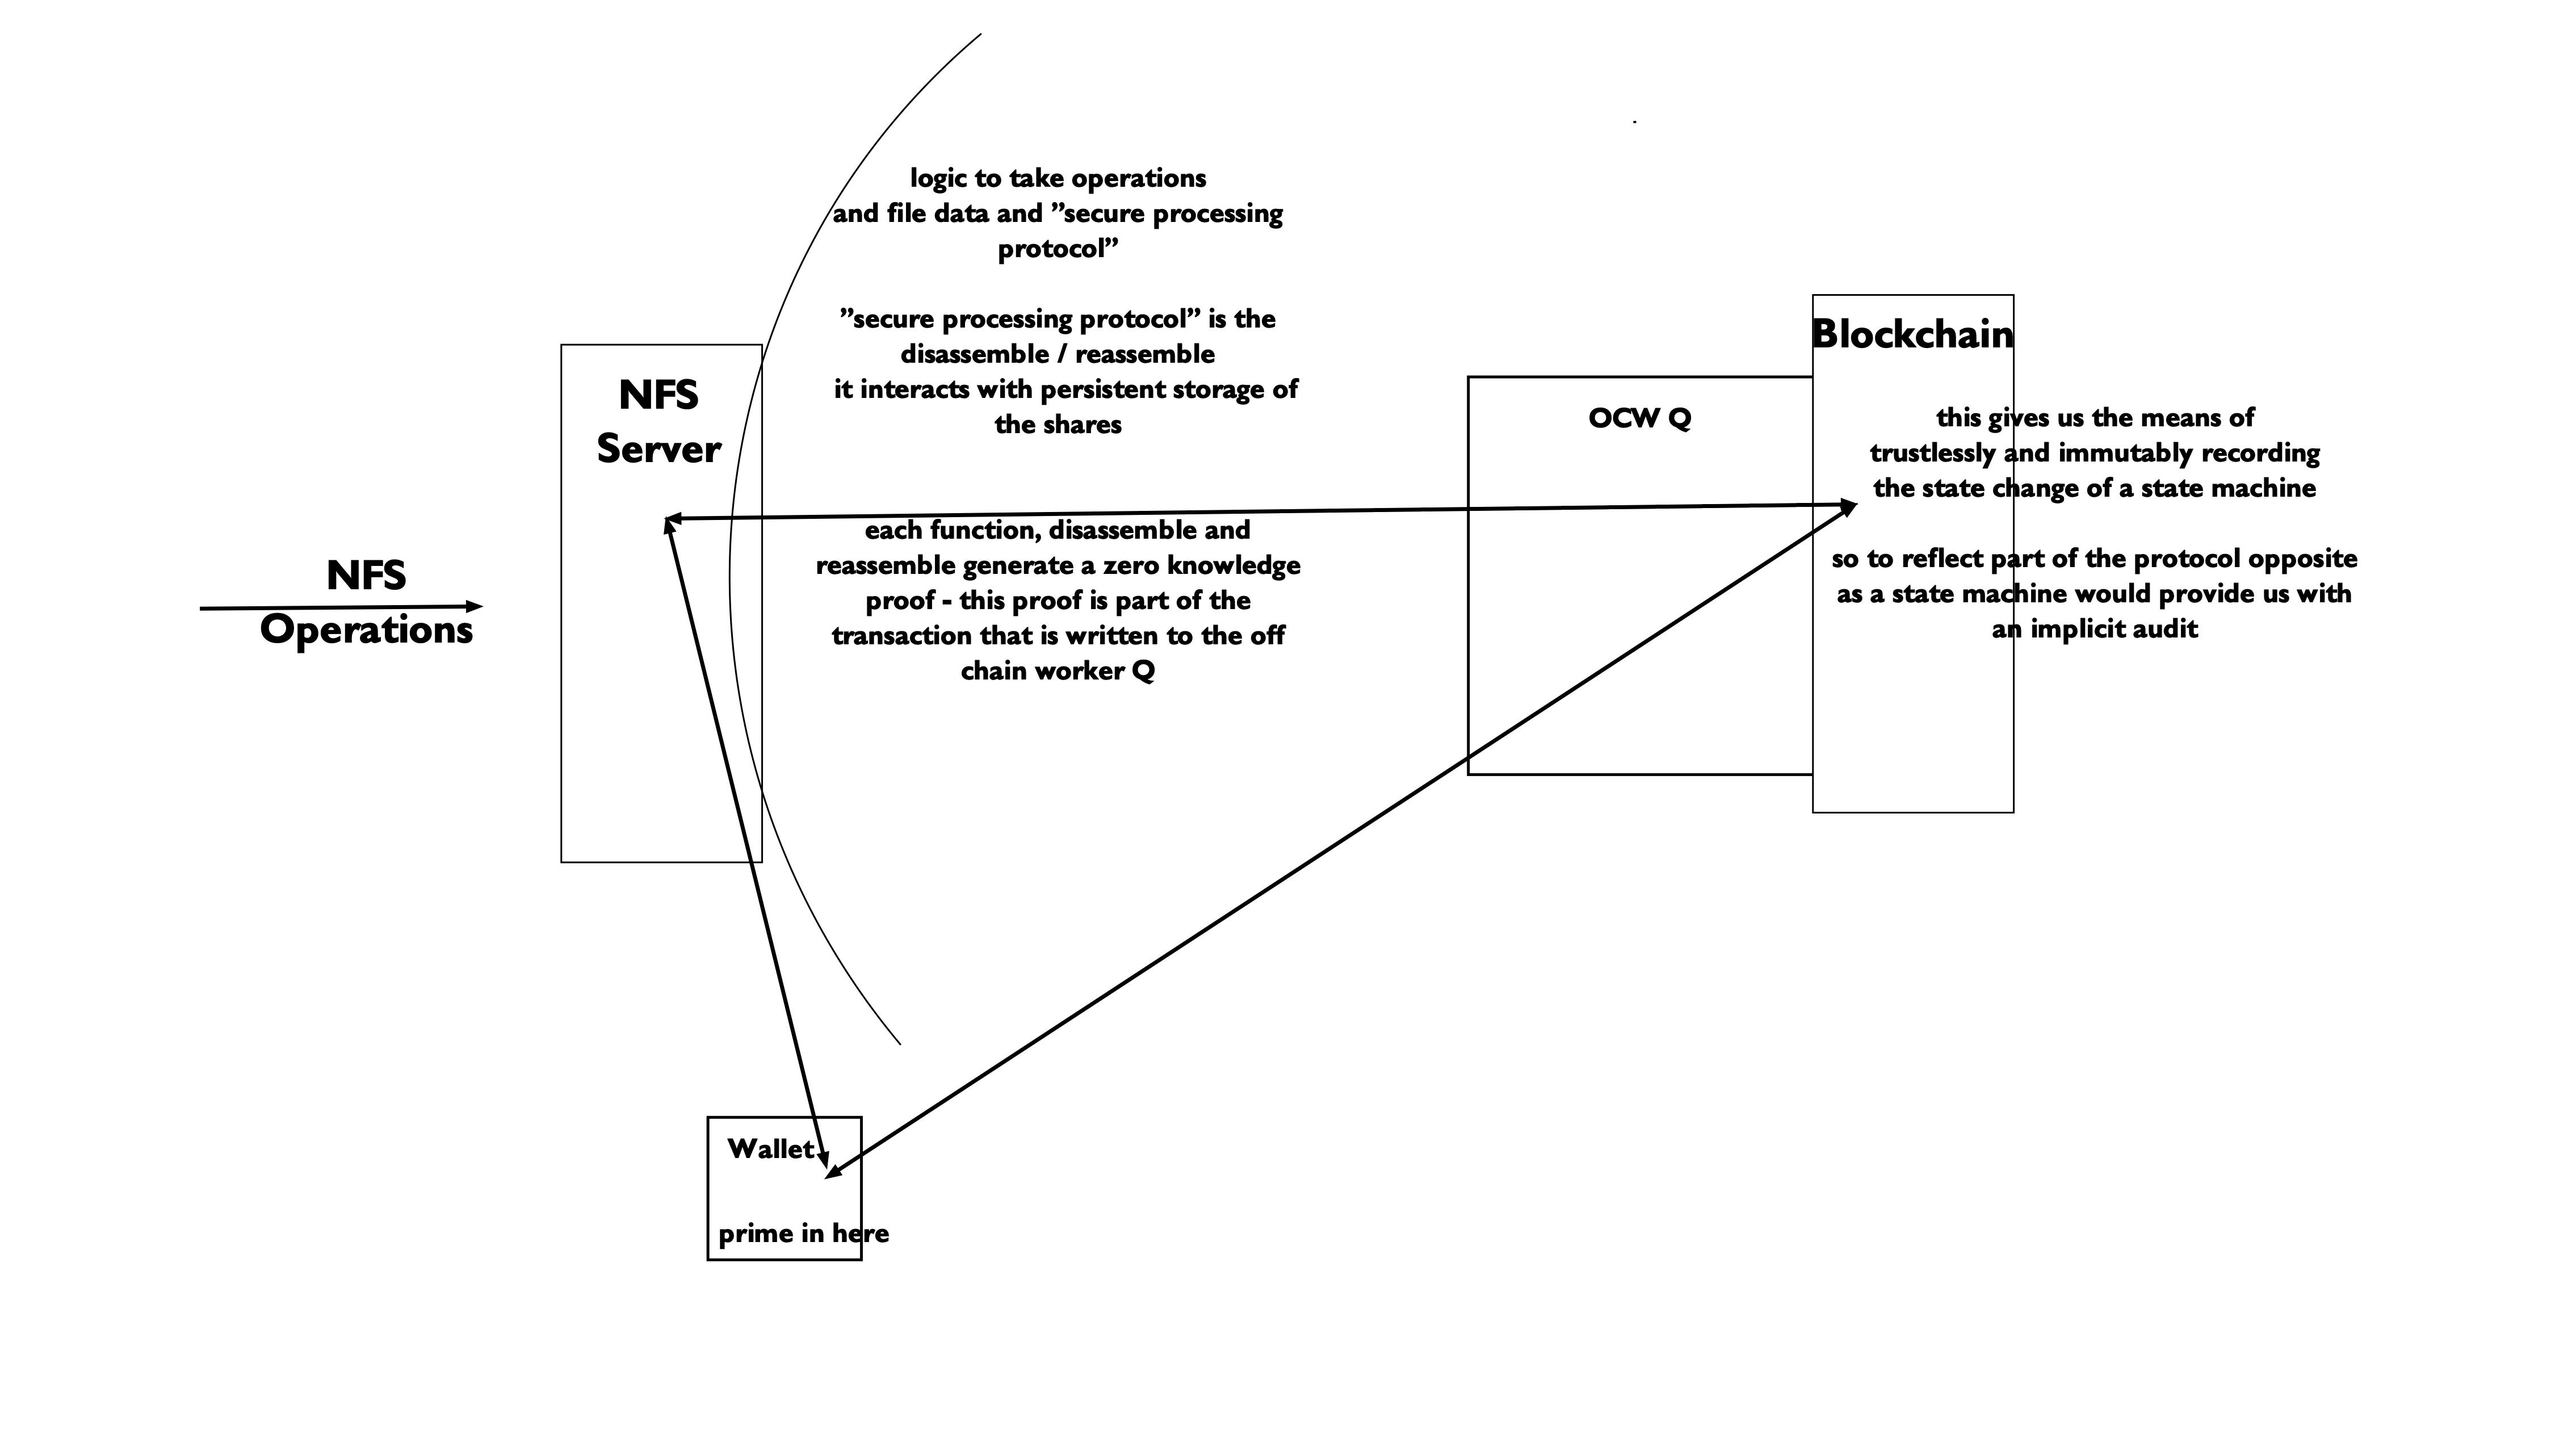
\includegraphics[width=1.2\textwidth]{NFS-polkadot-architecture.jpg}
    \caption{Overview}
    \label{fig:image1}
\end{figure}

This setup aims to balance the security and immutability benefits of blockchain with the performance requirements of a high-load filesystem.

Our approach of using off-chain aggregation to handle the computationally intensive Shamir's Secret Sharing operations while maintaining an immutable audit trail on
the blockchain is strategically sound for several reasons:
\begin{itemize}
\item Scalability: By offloading the Shamir operations to an off-chain queue, we reduce the load on the blockchain, allowing it to handle more transactions and operate
more efficiently. This is crucial for maintaining high performance as the system scales.
\item Security and Immutability: The blockchain still records all critical operations, providing an immutable audit trail of file access and share reassembly. This meets
the security requirements for sensitive data handling and compliance needs.
\item Asynchronous Processing: Handling Shamir operations off-chain and allowing the blockchain to process these operations asynchronously can significantly improve the
overall responsiveness and user experience of the system.
\item Flexibility: This architecture provides flexibility in managing the balance between immediate data processing needs and the slower, immutable record-keeping process
of the blockchain.
\end{itemize}
However, there are a few considerations and potential challenges, mainly due to the general case of off-chain processing:
\begin{itemize}
\item Complexity: The integration between off-chain and on-chain components adds complexity to the system, which might increase the potential for bugs and require more
robust testing and maintenance strategies.
\item Consistency and State Management: Ensuring that the off-chain state (Shamir shares) and the on-chain state (audit logs) remain consistent can be challenging.
Mechanisms must be in place to handle discrepancies and failures.
\item Security of Off-Chain Components: While the blockchain itself is secure, the off-chain components must also be secured, as they handle sensitive operations and data.
\item Latency and Timing Issues: Depending on how the off-chain queue is managed, there might be latency or timing issues in how quickly state transitions are reflected
on the blockchain, which could affect the timeliness of the audit trail.
\item Overall, if these challenges are addressed, this approach could effectively leverage the strengths of both off-chain processing and blockchain technology to
create a robust, scalable, and secure system.
\end{itemize}

That said, in the Polkadot ecosystem, you can integrate an off-chain queue more closely with the blockchain process using Substrate's off-chain features. Specifically,
Substrate provides a framework for off-chain workers (OCWs) that can perform computations and manage data off the main blockchain but still within the blockchain
node's environment. This allows for a more seamless integration between on-chain and off-chain processes, mitigating many of the issues cited above.

\subsection{How Off-Chain Workers Can Help}\label{sec:headings}
Off-chain Workers (OCWs) in Substrate run asynchronously and independently of the block production process. They can be triggered after each block is finalized and can communicate
with external services, perform heavy computations, or manage queues. Here's how you can leverage OCWs for our needs:
\begin{itemize}
\item Off-Chain Storage: OCWs can utilize Substrate's off-chain storage to temporarily store data before it is committed to the blockchain. This storage is local to each
node and is not consensus-critical, making it a good candidate for our off-chain queue.
\item Data Aggregation: OCWs can aggregate data from the off-chain queue and prepare it for submission to the blockchain. This can include batching operations or
performing preliminary computations necessary before updating the on-chain state. We should consider if we batch to save gas feees.
\item Scheduled Tasks: OCWs can be scheduled to run at specific intervals or in response to specific events, allowing for regular processing of the queue.
\item Secure Data Handling: While OCWs operate off-chain, they still maintain a high level of security and can utilise cryptographic functions provided by
Substrate to ensure data integrity and security.
\end{itemize}

\subsection{Implementing an Off-Chain Queue with OCWs}\label{sec:headings}
Here's a basic outline of how we will implement this:
\begin{itemize}
\item Modify the NFS Server: Adjust our NFS server to write operations related to Shamir's Secret Sharing into the off-chain storage managed by OCWs.
\item Develop Off-Chain Workers: Implement OCWs that periodically read from this off-chain storage, process the data as needed, and prepare transactions to update
the on-chain state.
\item Submit Transactions: After processing, OCWs can sign and submit transactions to the blockchain to record the final state or results of operations.
\item Error Handling and Retry Logic: Implement robust error handling and retry mechanisms in OCWs to manage failures in data processing or transaction submission.
\end{itemize}

This integration allows us to maintain the benefits of blockchain while effectively managing performance-intensive operations, keeping the system scalable and efficient.

Using Off-Chain Workers (OCWs) in Substrate does address many aspects of the security concerns associated with off-chain components, but it's important to understandthe scope and limitations of this security enhancement.

\subsection{Security Benefits of OCWs}\label{sec:headings}
\begin{itemize}
\item Isolation and Encapsulation: OCWs operate within the blockchain node's environment but are isolated from the core consensus-critical processes. This encapsulation
helps in minimizing the risk of off-chain activities affecting the blockchain's integrity directly.
\item Access to Cryptographic Functions: OCWs have access to Substrate's cryptographic functions, allowing them to securely sign transactions, verify signatures, and
handle sensitive data securely. This is crucial for maintaining the authenticity and non-repudiation of the off-chain data before it's submitted to the blockchain.
\item Controlled Interaction with Blockchain: OCWs can only interact with the blockchain through well-defined interfaces, specifically through submitting signed
transactions. This controlled interaction reduces the risk of unauthorized or malicious modifications to the blockchain state.
\end{itemize}

\subsection{Limitations and Remaining Security Concerns}\label{sec:headings}
\begin{itemize}
\item Node-Level Security: Since OCWs run on individual nodes, the security of each node becomes crucial. If a node is compromised, the OCWs running on that node
could potentially be manipulated. Ensuring the security of the hardware and operating environment of nodes is essential.
\item Data Transmission Security: While OCWs can securely handle data at the node, the transmission of data between nodes or from external sources to nodes needs to be
secured separately, typically using secure communication protocols like TLS.
\item Off-Chain Data Storage: Data stored off-chain, even temporarily, is not protected by the blockchain's consensus mechanisms. This data could be at risk if not
properly encrypted or if the storage medium is not secure.
\item Dependency on External Data and Services: If OCWs rely on external data or services, the security and reliability of these external components can impact the
overall system. For instance, data feeds or APIs that OCWs interact with need to be secure and trustworthy. Inour case i believe we are ok here.
\end{itemize}
\subsection{Mitigation Strategies}\label{sec:headings}
\begin{itemize}
    \item Node Security: We should mplement robust security measures for the nodes, including secure boot mechanisms, operating system hardening, and intrusion detection systems.
    \item Data Encryption: Encrypt sensitive data handled by OCWs both in transit and at rest, using strong encryption protocols.
    \item Regular Audits and Updates: Regularly audit the code and security infrastructure of OCWs and update them to patch any vulnerabilities.
    \item Redundancy and Consensus: For critical operations, consider having multiple OCWs across different nodes perform the same computations and use a consensus
    mechanism among them before submitting transactions to the blockchain.
\end{itemize}

In summary, while OCWs enhance the security of off-chain components by leveraging the blockchain node's capabilities, they do not eliminate all security risks.
A comprehensive security strategy that addresses both on-chain and off-chain components is essential for maintaining the overall security of the system.

\subsection{Integrity of Blockchain nodes}\label{sec:headings}
Given the scenario where users access the NFS Server using a Polkadot.js wallet containing a Shamir prime for decrypting their files, ensuring the integrity
of the blockchain nodes used is crucial. A streamlined approach to achieve this is outlined here, focusing on user registration and session validation through
the blockchain:
\begin{itemize}
\item User Registration on the Blockchain:
\begin{itemize}
    \item User Wallet: Each user registers on the blockchain via their Polkadot.js wallet. This registration can include their public key and any other relevant identifiers.
    \item Smart Contract: Implement a smart contract on the blockchain that handles user registrations. This contract stores user details securely and can be queried to
verify user identities. So this contract is the general RBAC contract.
\end{itemize}
\item Session Initialization:
\begin{itemize}
    \item Session Token: When a user accesses the NFS Server, they initiate a session by creating a session token or similar credential, which is then signed using their
    private key (from their wallet).
    \item Blockchain Verification: This token is sent to the blockchain (via a transaction or a direct smart contract call), where it's verified against the registered
    user details.
\end{itemize}
\item Filesystem Verification:
\begin{itemize}
    \item Smart Contract Query: Before allowing access to any files, the NFS Server queries the blockchain to verify the session token against the active user sessions
    registered in the smart contract.
    \item Access Control: If the session token is valid and matches the registered details on the blockchain, the NFS Server grants access to the user's files. If not,
    access is denied.
\end{itemize}
\item Blockchain Node Integrity:
\begin{itemize}
    \item Node Verification: To ensure the NFS Server is interacting with the correct blockchain nodes, use a list of trusted nodes maintained either in a secure
    configuration file or through a decentralized registry on the blockchain itself.
    \item TLS and Certificates: Secure communications between the NFS Server and the blockchain nodes using TLS, where each node presents a certificate that the NFS
    Server can verify against a list of trusted certificates.
\end{itemize}
\end{itemize}

This approach leverages blockchain for user authentication and session management, ensuring that the NFS Server interacts only with verified users and trusted
blockchain nodes, thereby enhancing the overall security and integrity of the system.

\subsection{Attesting to the Shamir steps}\label{sec:headings}
ZKPs can be used to validate transactions on the blockchain without revealing the underlying data that generated these transactions. A proof could be generated to
confirm that a file operation was correctly performed according to the Shamir's Secret Sharing protocol, without revealing the content of the files or the shares themselves.

Introducing zero-knowledge proofs (ZKPs) to verify file operations performed according to Shamir's Secret Sharing protocol without revealing the content of the files or the
shares themselves involves several steps. Here's how we can integrate this intoour architecture:

\begin{itemize}
\item Define the ZKP Scheme
First, you need to define the specific ZKP scheme that will be used to verify the operations. This involves:
\begin{itemize}
\item Choosing the right type of ZKP: Depending on our needs, you might choose zk-SNARKs, zk-STARKs, or another variant. zk-SNARKs are widely used due to their efficiency
in verification times but require a trusted setup. zk-STARKs, on the other hand, do not require a trusted setup and are post-quantum secure but are generally larger in size.
\item Creating the circuit: Define a computational circuit that represents the logic of Shamir's Secret Sharing operations. This circuit will be used to generate and
verify proofs. A circuit is required for disassemble and a circuit for reassembly.
\end{itemize}
\item Integration Points
\begin{itemize}
\item During File Operations: Integrate the generation of ZKPs into the process where files are split into shares or reassembled. This can be done on the client side
(in the user's environment) or by the off-chain workers if they handle such operations.
\item Verification by Smart Contract: Deploy a smart contract capable of verifying the proofs submitted along with transactions that record file operations on the
blockchain. This contract checks the validity of the operations without needing to see the underlying data.
\end{itemize}
\item Implementation Steps
\begin{itemize}
\item Proof Generation: When a file is split or shares are combined, the corresponding ZKP is generated. This proof attests that the operation was performed correctly
according to the rules defined in the computational circuit.
\item Submitting Proofs to Blockchain: Along with recording the operation on the blockchain, the proof is also submitted. This can be part of the transaction data.
\item Smart Contract for Proof Verification: The smart contract will use the ZKP verification algorithm to ensure the proof is valid. If the proof is valid, the operation
is recorded as successful; otherwise, it is rejected.
\end{itemize}
\item Security and Privacy Considerations
\begin{itemize}
\item Confidentiality: Ensure that no sensitive data is leaked during proof generation or verification. The ZKP should only prove the correctness of the operation,
not reveal any data.
\item Efficiency: Consider the computational and storage overhead introduced by ZKPs. Optimize the ZKP setup to balance security, privacy, and performance.
\end{itemize}
\end{itemize}

\section{Architecture Summary}\label{sec:page-layout}
Core components comprise:
\begin{itemize}
\item NFS Server: Manages secure file storage and access, utilising Shamir's Secret Sharing to split file information into shares.
\item Polkadot.js Wallet: Used by users to store their unique Shamir prime and interact with the blockchain.
\item Bespoke Blockchain (Built on Polkadot Substrate): Custom blockchain that models Shamir's Secret Sharing operations as state transitions. This blockchain
uses smart contracts for user registration and session management, and integrates off-chain workers for efficient processing.
\item Smart Contracts and Off-Chain Workers: Smart contracts handle user registration and session management. Off-chain workers process Shamir operations off-chain to
enhance performance and then queue these operations for asynchronous processing on the blockchain.
\item Zero-Knowledge Proofs (ZKPs): Used to verify the correctness of Shamir's Secret Sharing operations (disassembly and reassembly) without revealing the content of
the files or the shares themselves.
\end{itemize}

Workflow steps:
\begin{itemize}
\item User Registration:
\begin{itemize}
\item Users register on the blockchain via their Polkadot.js wallet, providing necessary credentials and their public key.
\item Registration details are securely stored in a smart contract on the blockchain.
\end{itemize}
\item Session Management:
\begin{itemize}
\item Users initiate sessions by creating a session token signed with their private key when accessing the NFS Server.
\item This token is verified against registered details on the blockchain via a smart contract.
\end{itemize}
\item File Access and Shamir Operations:
\begin{itemize}
\item Upon successful session verification, users can access and operate on their files.
\item File operations involve Shamir's Secret Sharing, where file data is split or combined using the user's part of the key from their wallet.
\item Each operation (splitting or combining shares) corresponds to a state transition in the bespoke blockchain, recorded and managed by the blockchain's state machine.
\end{itemize}
\item Zero-Knowledge Proof Generation and Verification:
\begin{itemize}
\item During file operations, ZKPs are generated to prove that operations were performed correctly according to Shamir's Secret Sharing protocol.
\item Proofs are submitted along with the state transition data to the blockchain via OCWs.
\item Smart contracts on the blockchain verify these proofs to ensure the integrity and correctness of the operations without accessing the actual data.
\end{itemize}
\item Off-Chain Workers:
\begin{itemize}
\item Off-chain workers process Shamir operations and ZKP generation off-chain to enhance performance.
\item These operations, along with their proofs, are then queued and asynchronously processed on the blockchain, ensuring efficient and scalable handling of data-intensive tasks.
\end{itemize}
\item Blockchain Node Integrity and Security:
\begin{itemize}
\item The NFS Server communicates only with verified blockchain nodes, ensuring node integrity through a list of approved nodes or certificates.
\item All communications are secured using TLS.
\end{itemize}
\end{itemize}

Security Features include:
\begin{itemize}
\item Immutable Audit Trails: The blockchain provides an immutable record of all Shamir operations as state transitions, along with ZKP verifications,
enhancing transparency and security.
\item Decentralized Trust: Utilizes blockchain for decentralized security, reducing the risk of tampering and reliance on a single point of failure.
\item Encrypted Communications: Uses TLS for secure communication between the NFS Server and blockchain nodes.
\item Role-Based Access and Multi-Factor Authentication: Ensures that only authorized users can access their files and make configuration changes.
\end{itemize}

This architecture effectively integrates the security and immutability of blockchain technology with the computational efficiency provided by off-chain workers
and the privacy-preserving capabilities of zero-knowledge proofs, specifically tailored to manage the complexities of Shamir's Secret Sharing in a file storage environment.

\bibliography{blockchain}
\bibliographystyle{plainnat}

\end{document}
